\documentclass[11pt,oneside]{scrartcl}

\usepackage[a4paper,margin=1in]{geometry}
\usepackage[T1]{fontenc}
\usepackage[utf8]{inputenc}
\usepackage{newtxtext,newtxmath}
\usepackage{microtype}
\usepackage{setspace}
\usepackage{graphicx}
\usepackage{booktabs}
\usepackage{tabularx}
\usepackage{array}
\usepackage{amsmath}
\usepackage{caption}
\usepackage{xcolor}
\usepackage{hyperref}
\usepackage{enumitem}
\usepackage{fancyhdr}
\usepackage{titlesec}
\usepackage{float}
\usepackage{longtable}

\hypersetup{
  colorlinks=true,
  linkcolor=black,
  urlcolor=blue!60!black,
  citecolor=black,
  pdftitle={Store-Level Time Series Forecasting of Restaurant Visitors Using ARIMAX}
}

\definecolor{titleblue}{HTML}{183A5A}
\definecolor{rulegray}{HTML}{B8C2CC}

\setstretch{1.15}
\setlength{\parindent}{0pt}
\setlength{\parskip}{0.6em}
\captionsetup{font=small,labelfont=bf}

\titleformat{\section}
  {\Large\bfseries\color{titleblue}}
  {\thesection.}{0.6em}{}
\titleformat{\subsection}
  {\large\bfseries\color{titleblue}}
  {\thesubsection}{0.6em}{}

\pagestyle{fancy}
\fancyhf{}
\fancyhead[L]{\footnotesize Store-Level Restaurant Visitor Forecasting}
\fancyhead[R]{\footnotesize \thepage}
\renewcommand{\headrulewidth}{0.4pt}
\renewcommand{\footrulewidth}{0pt}

\begin{document}

\begin{center}
{\LARGE\bfseries Store-Level Time Series Forecasting of Restaurant Visitors Using ARIMAX\par}
\vspace{0.5em}
{\large\itshape A Detailed Empirical Report Based on the Recruit Restaurant Visitor Forecasting Dataset\par}
\vspace{1em}
\color{rulegray}\rule{\textwidth}{0.8pt}
\end{center}

\begin{center}
\begin{tabular}{>{\bfseries}p{0.25\textwidth}p{0.65\textwidth}}
Final modelling notebook: & \texttt{notebooks/03\_final\_store\_level\_forecasting.ipynb} \\
Implemented comparison: & Seasonal Naive lag-7 baseline versus store-level ARIMAX \\
Forecasting unit: & $\texttt{air\_store\_id} \times \texttt{visit\_date}$ \\
Main evaluation: & pooled observed store-date RMSLE on the final chronological holdout \\
\end{tabular}
\end{center}

\vspace{0.5em}

\textbf{Scope statement.}
This report presents only the methods and results implemented in the final project pipeline. It does not report or rank models that were not part of the final store-level notebook. The strongest claim is deliberately narrow: ARIMAX is evaluated against the implemented Seasonal Naive benchmark using pooled store-date RMSLE in the final chronological holdout, with one lightweight expanding-window validation fold as supporting evidence.

\section*{Abstract}
This paper studies daily restaurant visitor forecasting using the Recruit Restaurant Visitor Forecasting dataset. The implemented comparison is deliberately focused on a weekly Seasonal Naive lag-7 benchmark versus a store-level ARIMAX model. The forecasting unit is $\texttt{air\_store\_id} \times \texttt{visit\_date}$, and the main evaluation metric is pooled observed store-date RMSLE on the final chronological holdout.

The final project follows the Kaggle prediction logic at the store-date level: the target is the number of visitors for each \texttt{air\_store\_id} on each date, rather than one aggregate visitor series for all restaurants combined. The central research question is whether a store-level ARIMAX model that uses weekly seasonality and economically meaningful exogenous variables can improve forecast accuracy relative to a simple weekly Seasonal Naive benchmark.

The theoretical framework treats restaurant demand as an operational decision problem under uncertainty. Daily demand is shaped by three mechanisms: persistence from recent store-specific demand, calendar-driven seasonality, and observable leading indicators such as reservations and holidays. The empirical pipeline constructs store-level daily series for 814 AIR stores, creates variables for holidays, weekends, Golden Week, and reservations, and evaluates forecasts on the final holdout window from 15 March 2017 to 22 April 2017. The baseline is Seasonal Naive with lag 7. The final model is ARIMAX$(1,1,1)(1,1,1)[7]$ estimated separately by store with exogenous regressors.

Over 31{,}476 observed store-date holdout rows, ARIMAX reduces RMSLE from 0.9622 to 0.8122, a 15.6\% improvement relative to the baseline, and outperforms the baseline for 79.1\% of evaluated stores. A lightweight expanding-window validation fold provides additional support: when trained through 31 January 2017 and tested on 1--7 February 2017, ARIMAX reduces RMSLE from 0.9327 to 0.7317, a 21.6\% improvement. The findings support the view that restaurant forecasting is more appropriate at the store level and should incorporate calendar information and reservation signals that reveal demand before the visit date, rather than relying only on repeated weekly history.

\section{Introduction}
Restaurant managers must make daily staffing, inventory, and capacity decisions before realised demand is fully observed. If the forecast is too low, the restaurant may face long waiting times, overworked staff, stock-outs, and lower customer satisfaction. If the forecast is too high, the restaurant may waste labour hours and perishable ingredients. Visitor forecasting is therefore not merely a technical prediction exercise. It is an operational problem of allocating limited resources under uncertainty, where forecast quality matters because it shapes decisions taken before demand is known.

This report addresses a deliberately narrow question: can a store-level ARIMAX model using calendar and reservation information forecast daily restaurant visitors more accurately than a simple weekly Seasonal Naive benchmark? The scope is intentionally precise. The project does not attempt to rank all possible time-series and machine-learning models. Instead, it evaluates a specific hypothesis motivated by the economics of restaurant demand: because demand is shaped by weekly routines, calendar effects, and advance reservations, a model that combines time-series dynamics with exogenous demand signals should outperform a benchmark that only repeats the previous week's observed pattern.

The empirical setting is the Recruit Restaurant Visitor Forecasting dataset, which contains visitor counts, reservation records, store information, and calendar variables for restaurants in Japan. The final modelling notebook uses 814 AIR stores and evaluates 812 stores after applying the final modelling requirements. The final chronological holdout runs from 15 March 2017 to 22 April 2017. The unit of analysis is a store-date row. This point is central to the design. The project is not forecasting one aggregate market-level series. It is forecasting daily demand for each individual store, which matches the real decision problem faced by restaurant operators and platforms.

Within that scope, the report makes four contributions. First, it aligns the empirical design with the operational prediction task by using store-level daily forecasting rather than aggregate forecasting. Second, it compares a transparent weekly benchmark with a fixed store-level ARIMAX specification that incorporates holiday, weekend, Golden Week, and reservation features. Third, it treats pooled store-date RMSLE as the primary accuracy metric while using the store-level win rate as supporting evidence that any gain is broadly distributed rather than concentrated in a few restaurants. Fourth, it separates supported forecasting claims from extensions that were not implemented or were only lightly tested, thereby keeping the argument proportional to the evidence.

The main result is straightforward. On the pooled final holdout, the Seasonal Naive baseline achieves RMSLE of 0.9622, while ARIMAX achieves RMSLE of 0.8122, a 15.6\% improvement. ARIMAX also performs better than the baseline for 79.1\% of evaluated stores. The project includes one lightweight expanding-window validation fold as supporting evidence. In that earlier split, ARIMAX reduces RMSLE from 0.9327 to 0.7317, a 21.6\% improvement. Taken together, these results support the view that store-level visitor demand contains information beyond repeated weekly seasonality alone. Weekly repetition remains useful, but it is incomplete. Forecasting improves when the model can also incorporate calendar information and reservation signals known before the visit date.

The rest of the report is organised as follows. Section 2 reviews the relevant forecasting literature and develops the theoretical framework. Section 3 describes the data, sample, variables, models, and evaluation strategy. Section 4 presents the main results. Section 5 discusses the economic interpretation, limitations, and future research directions. Section 6 concludes.

\subsection{Store-level forecasting as the decision unit}
The store-level design is not a cosmetic detail. It is central to the logic of the project. A restaurant platform may care about total demand across all restaurants, but operational decisions are made at the individual restaurant level. Staff are scheduled for a specific store, food is prepared in a specific kitchen, and service bottlenecks occur in a specific dining room. A forecast of total market demand could look accurate while still being useless for a manager if it hides large errors across individual restaurants.

This point also strengthens the use of pooled store-date RMSLE. The forecast task is not one series and one error per day; it is a panel of store-date forecasts. Pooled RMSLE treats each evaluated store-date row as an operational prediction unit and summarizes performance across that panel. The store-level win rate then adds a second diagnostic by asking whether ARIMAX improves broadly across stores or whether the pooled result is driven by a small subset of restaurants.

The store-level design does introduce a trade-off. Estimating separate ARIMAX models by store means each model has fewer observations than a pooled global model would have. Some stores have shorter histories and noisier demand patterns. However, this trade-off is reasonable for the goal of the report. Separate store-level models allow each restaurant's history to drive its own forecast, which is consistent with the theoretical view that restaurants differ in clientele, location, cuisine, operating schedule, and reservation behavior.

\section{Literature Review and Theoretical Framework}
\subsection{What the literature suggests about restaurant demand forecasting}
The literature relevant to this project spans three connected questions rather than one isolated modelling choice. First, how should restaurant demand be conceptualised as a time series? Second, what counts as a fair benchmark in a forecasting study? Third, when does external information justify moving from a pure univariate model to a dynamic regression design? Organising the review around these questions makes the empirical logic of the project clearer than simply listing forecasting methods in chronological order.

The first strand is the classical time-series literature. Box and Jenkins (1970) provide the core logic of ARIMA modelling, in which current values depend on autoregressive structure, differencing, and moving-average errors. For seasonal data, this framework naturally extends to seasonal autoregressive and seasonal moving-average components. Restaurant visitor counts are an intuitively suitable application because they are shaped by repeated weekly routines: Monday demand differs from Friday demand, and weekends often follow a different rhythm from workdays. The key implication is not merely that ARIMA exists, but that restaurant demand is unlikely to be well described as iid noise. It is a structured process with persistence and seasonality.

The second strand concerns forecasting benchmarks. Hyndman and Athanasopoulos (2021) argue that more complex models should be judged against simple and transparent alternatives, not against weak strawman comparators. This point is reinforced by large-scale forecasting evidence. Makridakis, Spiliotis, and Assimakopoulos (2018) show that simple statistical benchmarks remain difficult to beat across many forecasting environments. In the context of restaurant demand, this makes a weekly Seasonal Naive lag-7 forecast the relevant benchmark rather than a mean forecast or an unconditional trend rule. If demand has strong weekly structure, then repeating the same weekday from the previous week is already a serious forecasting standard. The empirical question is therefore not whether ARIMAX can outperform something trivial, but whether it can add value beyond a benchmark that already captures the most obvious seasonal pattern.

The third strand concerns dynamic regression and forecast-origin-valid exogenous information. ARIMAX models preserve the time-series structure of ARIMA while allowing predetermined external variables to shift the forecast. For restaurant demand, holidays and reservations are natural candidates for this role. A public holiday can alter leisure patterns even when recent weekly history looks ordinary. A reservation made before the visit date can reveal future demand that is not yet visible in the historical visitor series. The intervention-analysis tradition of Box and Tiao (1975) is relevant here because it formalises the idea that known external events should not simply be left in the error term when they are observable in advance.

A related methodological lesson concerns forecast evaluation. Hyndman and Koehler (2006) show that commonly used percentage-error measures can behave poorly when realised values are close to zero. That warning matters in store-level restaurant data, where some store-days have low visitor counts. The implication is broader than metric selection alone: evaluation should match the structure of the operational problem. If the decision unit is a store-date forecast, then the primary error metric should also respect that unit and avoid exaggerating the influence of low-count denominators.

Taken together, this literature creates a useful scholarly tension. On one side, simple weekly benchmarks are often strong and difficult to beat. On the other side, restaurant demand is not generated purely by its own past values, because known calendar conditions and pre-arrival reservations can shift demand before the visit date. The gap addressed in this project is therefore not the invention of a novel forecasting algorithm. It is the disciplined implementation of a store-level forecasting design that aligns three things simultaneously: the operational decision unit, the timing of usable information, and a fair benchmark rooted in weekly seasonality.

This is where the project makes its specific contribution. Much forecasting work can drift toward one of two mismatches: either it evaluates models on an aggregate series that is easier to predict but less useful for operations, or it introduces richer predictors without enforcing forecast-origin discipline strongly enough. The present report instead asks a narrower question with clearer empirical content: when forecasting is conducted at the store-date level, under chronological evaluation, and with reservation information restricted to what would have been known at the forecast origin, can a fixed store-level ARIMAX specification outperform a strong lag-7 Seasonal Naive benchmark? That is the precise question the remainder of the report takes to the data.

\subsection{Theoretical framework: demand under uncertainty}
The theoretical framework of the report treats restaurant visitor forecasting as a decision problem under uncertainty rather than as a purely statistical exercise. Managers must choose labour, ingredients, and table capacity before realised demand is known. In that setting, the value of forecasting comes from reducing mismatch between expected arrivals and prepared capacity. A better forecast does not create demand, but it improves the timing and scale of operational decisions made before demand is observed.

Within that decision problem, three channels are especially important. The first is store-specific persistence. A restaurant that has recently attracted many customers may continue to do so because of local reputation, cuisine type, location, habitual clientele, or short-run demand momentum. The second is calendar structure. Workdays, weekends, public holidays, and extended holiday periods change opportunity costs and leisure patterns, so demand is not equally likely on all dates. The third is advance demand revelation. Reservations are observed before the visit occurs and therefore provide direct information about future arrivals that is not fully contained in past visitor counts.

These channels map directly onto the empirical comparison in the project. Seasonal Naive lag 7 captures the simplest possible version of the calendar channel by repeating the same weekday from the previous week. ARIMAX captures that weekly structure through seasonal time-series terms while also incorporating calendar and reservation information as exogenous regressors. The model comparison therefore has a clear theoretical interpretation: if ARIMAX outperforms the weekly benchmark, then the additional channels carry predictive value beyond repeated weekly history alone.

The framework also constrains the type of claim the report is allowed to make. This is a forecasting design, not a causal identification design. Holiday indicators and reservation signals are included because they are known before the forecasted visit date and therefore belong in the forecast information set. The question is whether these variables improve prediction under realistic timing, not whether the report identifies their causal effect on visitor demand. This distinction is not cosmetic. It is what keeps the theory, variables, and empirical claim aligned.

\subsection{Hypothesis derived from the framework}
The theoretical framework implies one main hypothesis with a deliberately narrow scope: a store-level ARIMAX model that combines weekly seasonality with calendar and reservation variables should forecast daily visitors more accurately than a Seasonal Naive lag-7 benchmark. This is not a claim that ARIMAX is universally optimal or that it should dominate every forecasting alternative. It is a more disciplined claim: within the implemented design, ARIMAX should outperform the weekly benchmark if exogenous demand signals contain predictive information beyond last week's same-day demand.

That main hypothesis can be decomposed into three expectations that connect the theory to the empirical test:
\begin{enumerate}[label=H\arabic*:,leftmargin=2.5em]
  \item weekly seasonality is strong enough that a lag-7 benchmark provides a meaningful forecasting standard;
  \item calendar variables such as holidays and weekends provide predictive information beyond simple weekly repetition;
  \item reservation counts act as leading demand indicators and improve store-level visitor forecasts when incorporated into a dynamic regression model.
\end{enumerate}

Stating the hypothesis this way matters for two reasons. First, it makes the benchmark part of the theory rather than just a technical comparator. Second, it makes clear that the report is not trying to settle the broad question of which forecasting paradigm is best in general. It is testing whether one coherent store-level design, motivated by the economics of restaurant demand, can improve on a strong weekly standard under chronological evaluation.

\begin{table}[H]
\centering
\caption{Theoretical channels and empirical representation}
\begin{tabularx}{\textwidth}{>{\raggedright\arraybackslash}p{0.26\textwidth} >{\raggedright\arraybackslash}p{0.34\textwidth} >{\raggedright\arraybackslash}X}
\toprule
Theoretical channel & Operational interpretation & Empirical representation \\
\midrule
Store-specific persistence & Demand is partly shaped by recent store-level history & ARIMA terms in ARIMAX \\
Weekly calendar structure & Customer behaviour differs by weekday and weekend & Seasonal period $= 7$ and \texttt{is\_weekend} \\
Holiday shocks & Public holidays can shift eating-out behaviour & \texttt{is\_holiday} and \texttt{is\_golden\_week} \\
Advance demand signal & Reservations reveal expected visitors before arrival & \texttt{log1p\_reserve} \\
\bottomrule
\end{tabularx}
\end{table}

\subsection{Testable implications of the framework}
The framework implies several empirical patterns that make the later evaluation interpretable rather than arbitrary. First, the Seasonal Naive model should be a meaningful baseline, not a trivial one. If weekly seasonality is genuinely strong, then last week's same weekday should already provide a reasonable first approximation of future demand. Second, ARIMAX should improve pooled RMSLE if calendar variables and reservation signals contain predictive information beyond weekly repetition. Third, the improvement should appear not only in the pooled metric but also across a substantial share of stores. A pooled gain without store-level consistency would be less persuasive because it could be driven by a narrow subset of high-volume or unusually predictable restaurants.

These expectations also explain why the report uses more than one summary statistic. Pooled RMSLE tests whether the final model lowers average log-scale error across the operational prediction rows. The store-level win rate tests whether the improvement is broadly distributed across the restaurant panel rather than concentrated in a few cases. The lightweight expanding-window fold tests whether the same directional advantage appears at another forecast origin, even though it is not a full rolling-origin validation design. Together, these criteria connect the empirical evidence back to the theory of the problem instead of treating evaluation as a purely technical afterthought.

\subsection{From theory to empirical design}
The empirical design follows directly from the theoretical structure of the problem. If restaurant demand contains persistence, then recent store-level history must be allowed to matter in the model. If it contains strong weekly seasonality, then both the benchmark and the final specification must reflect a seven-day cycle. If known calendar conditions and reservations shift demand before the visit date, then those variables belong in the forecasting information set rather than being treated as unexplained disturbances. If the relevant operational decision is made at the store-date level, then both modelling and evaluation should also be conducted at the store-date level rather than on an aggregate series.

This mapping matters because it shows that the final pipeline is not a collection of disconnected technical choices. The weekly Seasonal Naive model is the theoretical null model for repeated weekly structure. ARIMAX is the theoretical extension that allows predetermined external information to enter alongside internal dynamics. Chronological evaluation is required because forecasting is defined by information timing. Pooled RMSLE is appropriate because the target is a non-negative, heterogeneous count process observed across many stores. In that sense, the empirical design is not merely compatible with the theory; it is derived from it. The detailed operationalisation of variables, model choice, and predictive-use interpretation are presented in Section 3.

\section{Data and Methodology}
\subsection{Data source and final sample}
The empirical analysis uses the Recruit Restaurant Visitor Forecasting dataset, which combines restaurant visits, reservations, store characteristics, and calendar information. In the original Kaggle release, reservation data come from both the AIR and HPG platforms. The final project operationalises reservations by using AIR reservations together with mapped HPG reservations, thereby preserving the core forecasting role of reservations as pre-arrival demand signals while keeping the unit of analysis tied to AIR store identifiers.

The final sample begins with 814 AIR stores. Of these, 812 stores are evaluated in the final holdout and 2 are skipped because they do not satisfy the final modelling requirements. A key design choice is that each store series is built only over its observed date span rather than being padded with synthetic pre-history. Missing days inside that observed span are then filled as zero visitors in order to create the regular daily spacing required for both the lag-7 benchmark and the ARIMAX specification.

The global visit range in the final notebook runs from 1 January 2016 to 22 April 2017, but the effective modelling window differs by store because each series begins at its own first observed date. The final training period ends on 14 March 2017, and the final holdout runs from 15 March 2017 to 22 April 2017. The pooled holdout contains 31{,}476 observed store-date rows. This design is large enough to produce a meaningful pooled comparison while still preserving the chronological integrity of the forecasting problem.

\begin{table}[H]
\centering
\caption{Final sample definition}
\begin{tabular}{ll}
\toprule
Item & Final project value \\
\midrule
Forecasting unit & $\texttt{air\_store\_id} \times \texttt{visit\_date}$ \\
Stores total & 814 \\
Stores evaluated in final holdout & 812 \\
Stores skipped in final holdout & 2 \\
Global visit range & 2016-01-01 to 2017-04-22 \\
Final train end & 2017-03-14 \\
Final holdout window & 2017-03-15 to 2017-04-22 \\
Holdout observations & 31{,}476 pooled observed store-date rows \\
ARIMAX fitting failures & 0 \\
\bottomrule
\end{tabular}
\end{table}

\subsection{Data cleaning and feature construction}
Feature construction is organised around one central requirement: ARIMAX needs a regular time index. The final notebook therefore builds a daily frame for each store over that store's observed span. The dependent variable is daily visitors, and the transformed modelling target is \texttt{log1p\_visitors}. This transformation reduces skewness, handles zero counts naturally, and aligns the modelling scale with the report's preferred evaluation metric, RMSLE.

The reservation feature is constructed by aggregating reserved visitors at the store-date level and then applying \texttt{log1p}. The final reservation source combines AIR reservations with mapped HPG reservations. Conceptually, this variable matters because it represents information observed before the visit date rather than merely another lag of realised demand. The log transformation also reflects a practical forecasting intuition: the informational gain from reservations is likely to be nonlinear, especially at high counts.

The calendar regressors include \texttt{is\_holiday}, \texttt{is\_weekend}, and \texttt{is\_golden\_week}. These variables represent known information available prior to the forecasted date and therefore fit naturally into a forecasting design. The rule for filling missing days is equally important. The final notebook builds each store only within its observed date span, then fills internal missing dates as zero visitors. This should be understood as an operational panel-construction rule rather than as a literal claim that every missing raw-data date corresponds to true zero demand or confirmed closure.

The final notebook also caps holdout reservation regressors at the forecast origin, 14 March 2017. This is a critical leakage-control step because it prevents the model from using reservation records that would not have been known when the holdout forecast was generated. In other words, the reservation variable is treated as a valid information set component rather than as a backfilled future signal.

\begin{table}[H]
\centering
\caption{Core variables used in the final model}
\begin{tabularx}{\textwidth}{>{\raggedright\arraybackslash}p{0.22\textwidth} >{\raggedright\arraybackslash}p{0.38\textwidth} >{\raggedright\arraybackslash}X}
\toprule
Variable & Definition in the project & Theoretical reason \\
\midrule
\texttt{visitors} & Daily observed visitors for each \texttt{air\_store\_id} & Operational demand to be forecast \\
\texttt{log1p\_visitors} & $\log(1+\texttt{visitors})$ & Stabilises scale and matches RMSLE \\
\texttt{is\_holiday} & Public-holiday indicator & Captures abnormal calendar demand \\
\texttt{is\_weekend} & Weekend indicator & Captures recurring non-working-day behaviour \\
\texttt{is\_golden\_week} & Golden Week indicator & Controls for a major Japanese holiday period \\
\texttt{log1p\_reserve} & $\log(1+\texttt{reserved visitors})$ by store-date & Leading indicator of future arrivals \\
\bottomrule
\end{tabularx}
\end{table}

\subsection{Operationalisation of theoretical channels}
The theoretical framework becomes operational only when each channel is represented by variables with a clear forecasting role. The target variable, daily visitors, is realised restaurant demand at the store-date level. Because visitor counts are non-negative and right-skewed, the model uses the \texttt{log1p} transformation. This choice is not only convenient statistically; it also aligns the modelling scale with RMSLE, which measures error on a comparable log scale and reduces the dominance of very large stores.

Formally, if $y_{i,t}$ denotes observed visitors for store $i$ on date $t$, the transformed target is
\[
z_{i,t} = \log(1+y_{i,t}).
\]
Throughout the report, $y_{i,t}$ denotes visitor counts on the original scale, while $z_{i,t}$ denotes the log-transformed series used for estimation. This transformation preserves the non-negativity of the original count process while moving the estimation problem onto a scale that is less dominated by a small number of very large observations.

The calendar variables correspond to distinct demand mechanisms. The variable \texttt{is\_weekend} represents predictable changes in customer opportunity cost and leisure time. The variable \texttt{is\_holiday} represents known public-holiday disruptions to ordinary weekly patterns. The variable \texttt{is\_golden\_week} represents a Japan-specific holiday period that is theoretically relevant because it is associated with travel and leisure activity. The reservation variable, \texttt{log1p\_reserve}, is the clearest operational measure of advance demand revelation because it captures information about expected future attendance before the visit date arrives.

The distinction between lagged demand and reservations is especially important conceptually. Lagged visitors summarise what happened in the past, while reservations describe commitments or intentions about a future date. Seasonal Naive can only repeat last week's same weekday and therefore cannot react when future-date bookings shift materially. ARIMAX can adjust the forecast when reservation information is already known at the forecast origin. This is the strongest theoretical reason why a dynamic regression model can plausibly outperform a weekly benchmark even when the weekly benchmark is already strong.

\begin{table}[H]
\centering
\caption{Operationalisation of theoretical channels in the final project}
\begin{tabularx}{\textwidth}{>{\raggedright\arraybackslash}p{0.2\textwidth} >{\raggedright\arraybackslash}p{0.28\textwidth} >{\raggedright\arraybackslash}p{0.22\textwidth} >{\raggedright\arraybackslash}X}
\toprule
Theoretical channel & Operational meaning & Empirical representation & Expected forecasting role \\
\midrule
Store-specific persistence & Recent store demand contains information about future demand & AR and MA terms in ARIMAX & Captures dynamic dependence within each store \\
Weekly seasonality & Demand differs systematically across weekdays & Seasonal period 7 and Seasonal Naive lag 7 & Captures repeated weekly rhythm \\
Calendar structure & Weekends and public holidays change behaviour & \texttt{is\_weekend}, \texttt{is\_holiday}, \texttt{is\_golden\_week} & Allows known date effects to shift forecasts \\
Advance demand revelation & Reservations reveal future demand before arrival & \texttt{log1p\_reserve} from AIR + mapped HPG & Adds leading information unavailable to the naive benchmark \\
Scale heterogeneity & Restaurants differ greatly in visitor volume & \texttt{log1p\_visitors}, RMSLE & Makes errors more comparable across stores \\
\bottomrule
\end{tabularx}
\end{table}

\subsection{Model 1: Seasonal Naive lag-7 baseline}
The baseline model is Seasonal Naive with lag 7. For each store, the forecast for a date is based on the observed visitor count from the same weekday in the previous week. This benchmark is deliberately strong rather than merely convenient. It directly captures weekly seasonality, which is one of the most persistent and economically plausible regularities in restaurant demand. Its strength is transparency and low specification risk; its limitation is that it assumes last week's pattern is sufficient even when calendar conditions or reservation information imply otherwise.

In formal terms, the Seasonal Naive benchmark for store $i$ can be written as
\[
\hat{y}_{i,t\mid t-1} = y_{i,t-7},
\]
so the forecast for date $t$ is simply the realised demand from the same weekday one week earlier. The benchmark is therefore defined on the original visitor-count scale and later evaluated through the same pooled RMSLE criterion as the final model. In theoretical terms, this acts as a null model in which the dominant systematic component of demand is repeated weekly structure.

From a theoretical perspective, Seasonal Naive also serves as a null model. It encodes the claim that the main predictable component of restaurant demand is same-weekday repetition. This makes the benchmark especially useful in an academic forecasting comparison: the final model must demonstrate value beyond the most obvious seasonal mechanism already present in the data. If ARIMAX cannot outperform that weekly null, then its additional structure is not justified.

\subsection{Model 2: Store-level ARIMAX specification}
The final model is ARIMAX$(1,1,1)(1,1,1)[7]$, estimated separately for each store. The non-seasonal terms model short-run store-specific dynamics, while the seasonal component uses a seven-day period to capture weekly repetition. The exogenous regressors are \texttt{is\_holiday}, \texttt{is\_golden\_week}, \texttt{is\_weekend}, and \texttt{log1p\_reserve}. This specification corresponds closely to the theoretical framework developed in Section 2: persistence is handled by ARIMA dynamics, weekly structure is handled by the seasonal component, and predetermined demand signals are handled by the exogenous variables.

Using the backshift operator $B$, where
\[
By_t = y_{t-1},
\]
the ARIMAX family can be written compactly as
\[
\Phi(B^s)\phi(B)(1-B)^d(1-B^s)^D y_t
=
\beta'x_t + \Theta(B^s)\theta(B)\varepsilon_t,
\]
where $x_t$ is the vector of predetermined exogenous regressors, $s$ is the seasonal period, $\phi(\cdot)$ and $\theta(\cdot)$ are the non-seasonal autoregressive and moving-average polynomials, $\Phi(\cdot)$ and $\Theta(\cdot)$ are their seasonal counterparts, and $\varepsilon_t$ is the disturbance term. In the implemented model, $s=7$, $d=1$, and $D=1$, so the final store-level specification is
\[
\Phi(B^7)\phi(B)(1-B)(1-B^7) z_t
=
\beta'x_t + \Theta(B^7)\theta(B)\varepsilon_t,
\]
where $z_t=\log(1+y_t)$ and $x_t$ contains \texttt{is\_holiday}, \texttt{is\_golden\_week}, \texttt{is\_weekend}, and \texttt{log1p\_reserve}. The equation makes the theoretical structure explicit: differencing acts on the transformed demand process, autoregressive and moving-average terms capture internal dynamics, and the vector $\beta'x_t$ introduces predetermined external information into the forecast.

The order $(1,1,1)(1,1,1)[7]$ is used as a theoretically motivated fixed specification. The differencing terms address non-stationary level and seasonal patterns, the seven-day seasonality follows the dominant weekly structure identified in the exploratory analysis, and the low-order AR and MA terms provide a parsimonious representation that remains computationally feasible across more than 800 stores. The design is therefore justified by a balance of theory, runtime, stability, and interpretability rather than by exhaustive per-store tuning.

The differencing choices are especially important from a time-series perspective. The non-seasonal differencing term $d=1$ addresses the possibility that store-level visitor demand contains local level shifts or slow-moving trend behaviour that would make the undifferenced process non-stationary. The seasonal differencing term $D=1$ at period 7 addresses recurring weekly non-stationarity, which is plausible when weekdays differ systematically in level rather than only through short-run random variation. These terms therefore reflect a theoretical expectation about the stochastic structure of restaurant demand rather than an arbitrary modelling preference.

The differencing operators themselves can be written as
\[
(1-B)y_t = y_t-y_{t-1}
\]
and
\[
(1-B^7)y_t = y_t-y_{t-7}.
\]
The first removes local level variation, while the second removes recurring weekly level effects. The use of both operators therefore reflects a formal commitment to handling both ordinary and seasonal non-stationarity before interpreting the remaining dependence structure. In the implemented model, these operators are applied to the transformed process $z_t$, but the intuition is unchanged: the aim is to stabilise the series before modelling its residual dependence.

The low-order AR and MA components serve a related purpose. In ARIMA-family modelling, the goal is not to maximise in-sample fit mechanically, but to capture dependence with a specification that is rich enough to represent persistence and flexible enough to accommodate forecast errors, while remaining parsimonious enough to avoid unstable estimation. The final order should therefore be read as a disciplined dynamic representation rather than as a claim that every store shares identical micro-dynamics.

A common order across stores is imposed as a deliberate trade-off between local flexibility and comparative discipline. Allowing every store to have its own tuned ARIMA order might improve some individual forecasts, but it would also introduce a large model-selection layer, increase overfitting risk, and make the comparison with the benchmark less transparent. The implemented design therefore favours a coherent and reproducible forecasting framework over maximal per-store optimisation.

\begin{table}[H]
\centering
\caption{Implemented model comparison}
\begin{tabularx}{\textwidth}{>{\raggedright\arraybackslash}p{0.24\textwidth} >{\raggedright\arraybackslash}p{0.16\textwidth} >{\raggedright\arraybackslash}p{0.33\textwidth} >{\raggedright\arraybackslash}X}
\toprule
Model & Role & Information used & Main limitation \\
\midrule
Seasonal Naive lag 7 & Benchmark & Same weekday from previous week & Ignores reservations and holiday shocks \\
ARIMAX$(1,1,1)(1,1,1)[7]$ & Final model & Store history, weekly seasonality, holidays, weekends, Golden Week, reservations & Fixed order and limited validation windows \\
\bottomrule
\end{tabularx}
\end{table}

\subsection{Why ARIMAX is appropriate for this forecasting task}
A possible criticism is that different stores might prefer different ARIMA orders. That criticism is reasonable, but it does not invalidate the implemented design. The project chooses a fixed order as a trade-off between local optimality, comparability, runtime, and reproducibility. If every store had a separately tuned order, the project would introduce a second modelling layer: model selection for hundreds of individual stores. That could improve some store-level forecasts, but it would also increase complexity and overfitting risk.

A fixed order keeps the empirical question clean. The report is not asking whether the best possible ARIMA order can be found for every restaurant. It asks whether one coherent store-level dynamic regression specification, motivated by weekly seasonality and exogenous demand signals, can improve over a strong weekly benchmark. The common order makes stores comparable and allows the performance difference to be attributed to the overall modelling framework rather than to a complicated search procedure.

ARIMA would model each store's visitor series using only its own past values, differencing, and moving-average errors. That is appropriate when the target process can be treated as being generated mainly by its internal dynamics. For this project, however, that assumption is too narrow. The theoretical framework implies that restaurant demand is influenced not only by its own recent history, but also by information known outside the target sequence, especially calendar effects and reservations observed before the visit date. ARIMAX is therefore more appropriate because it preserves the time-series structure of ARIMA while allowing these predetermined demand signals to enter the forecast explicitly.

The same logic applies to stationarity and differencing. ARIMA-family models are built on the principle that non-stationary behaviour should be handled explicitly rather than ignored. In the present setting, non-stationarity can arise in at least two forms: store-level demand can shift over time because of changing popularity, local shocks, or evolving customer routines, and weekly demand can exhibit recurring seasonal non-stationarity if weekdays differ systematically in level. The inclusion of both non-seasonal and seasonal differencing therefore follows the logic of time-series theory: stabilise the stochastic process before interpreting its dynamic dependence.

The predictive interpretation of the regressors is equally important. This report is a forecasting study, not a causal identification study. Calendar indicators and reservations are included because they would have been known at the forecast origin and therefore belong in the valid forecasting information set. More reservations do not need a causal interpretation to be operationally useful; for forecasting purposes, it is enough that they reveal information about expected future demand before the visit date. This predictive framing is also why forecast-origin discipline matters so much in the implementation.

Taken together, these choices make the final ARIMAX structure a deliberate design decision rather than an ignored weakness. The model does not merely append external regressors to an unstructured series. It first addresses the time-series behaviour of the target through differencing, then models the remaining dependence through parsimonious AR and MA terms, and finally allows predetermined external information to shift the forecast. That sequence is faithful to the theoretical discipline of time-series analysis and helps explain why the report treats ARIMAX as an extension of ARIMA rather than just a feature-rich regression.

\subsection{Forecast-origin discipline and leakage control}
A central requirement in time-series forecasting is that the model must not use information unavailable at the time the prediction is made. Reservation data require particular care because each record contains both a reservation timestamp and a visit date. The final notebook therefore caps holdout reservation regressors at 14 March 2017 for the final holdout. In practice, this means the model does not use reservation information created after the training cutoff when generating holdout forecasts.

This leakage-control rule is not a minor implementation detail. Because \texttt{log1p\_reserve} is a leading indicator, it could inflate performance artificially if constructed without regard to forecast timing. By capping reservation inputs at the forecast origin, the project demonstrates that the exogenous regressor is being used as genuine pre-forecast information rather than as retrospectively observed future knowledge. This makes the comparison with Seasonal Naive not only stricter, but also more substantively credible.

The treatment of missing dates raises a related methodological issue. Both ARIMAX and the lag-7 baseline require a regular daily time index. The final project avoids synthetic pre-history padding and models each store only over its observed date span. Within that span, missing days are filled as zero visitors. This is a pragmatic modelling assumption that preserves regular spacing. It should not be interpreted more strongly than that: the procedure creates a usable forecasting panel, but it does not by itself identify whether each missing raw record reflects closure, true zero demand, or incomplete observation.

\subsection{Reproducibility}
The empirical results are reproducible from the final modelling notebook and the processed inputs stored in the repository. The notebook reads from \texttt{notebooks/processed\_data/}, writes corrected outputs to \texttt{output/}, and the final reported results rely on the corrected \texttt{\_v2} files rather than earlier intermediate experiments. The repository also includes a requirements file listing the core software dependencies. This organisation is intended to preserve evidentiary traceability by making clear which notebook, inputs, and outputs support the final claim.

\subsection{Evaluation strategy and metrics}
Because the data are time series, evaluation is conducted through chronological splitting rather than random sampling. The primary reported metric is pooled RMSLE over all observed store-date rows in the final holdout. This metric is central because the forecasting task itself is defined at the store-date level and because the holdout contains many restaurants observed over the same final test window. Pooling all evaluated store-date errors therefore provides one overall measure of forecasting performance across the operational prediction units.

Formally, if $y_j$ and $\hat{y}_j$ denote the observed and forecast visitor counts for evaluated store-date row $j$, pooled RMSLE is
\[
\mathrm{RMSLE}
=
\sqrt{
\frac{1}{n}
\sum_{j=1}^{n}
\left[
\log(1+\hat{y}_j)-\log(1+y_j)
\right]^2
}.
\]
This definition shows explicitly why the metric aligns naturally with the transformed modelling scale used in the final specification. The model is estimated on the log-transformed series, while the reported evaluation is expressed as the root mean squared distance between realised and forecast counts on that same log scale.

Chronological validation is necessary because the order of observations contains information. A random train--test split would be inappropriate: it could place later observations in the training set and earlier observations in the test set, creating an evaluation environment unlike the real forecasting problem. In practice, forecasts are always formed without knowledge of future realised demand. The final holdout therefore begins after the training period, and the lightweight validation fold also preserves temporal order.

RMSLE is particularly suitable because visitor counts are non-negative and heterogeneous across stores. A raw error of 10 visitors has a very different meaning for a restaurant that usually serves 15 visitors than for one that typically serves 120. Log-scale errors reduce the dominance of large stores, accommodate zeros through the \texttt{log1p} transformation, and reflect the fact that proportional misses are often more meaningful than raw absolute deviations in operational forecasting.

MAPE is retained only as a secondary metric. It is intuitive because it is expressed as a percentage, but it becomes unstable when actual visitor counts are small. For that reason, the main judgement of the report is based on RMSLE and the store-level win rate rather than on percentage errors alone. The final notebook also includes one lightweight expanding-window validation fold with training ending on 31 January 2017 and a test window covering 1 February to 7 February 2017. That fold is interpreted as a supporting validation check rather than as full rolling-origin cross-validation.

\subsection{Methodological safeguards}
The credibility of the project depends on four safeguards: chronological evaluation, a meaningful seasonal benchmark, a store-level forecasting unit, and reservation features capped at the training cutoff. Together, these safeguards make the final metrics interpretable and ensure that the supported conclusion remains aligned with the implemented design.

These safeguards matter because final metrics are persuasive only when the design that produced them is defensible. A strong benchmark prevents easy wins against weak comparators. Chronological evaluation prevents future information from contaminating the test period. The store-level forecasting unit keeps the empirical design aligned with the operational decision problem. Forecast-origin discipline prevents the reservation signal from becoming a form of hidden leakage. Together, these choices support a coherent time-series methodology rather than a loosely assembled predictive exercise.

\subsection{Implementation pipeline summary}
Table~7 summarises the implemented pipeline from data integration to chronological evaluation. Its purpose is not to add a second methods narrative, but to condense the empirical workflow into one place and show how the final implementation maps onto the forecasting design described above.

\begin{table}[H]
\centering
\caption{End-to-end forecasting pipeline in the final project}
\begin{tabularx}{\textwidth}{>{\raggedright\arraybackslash}p{0.2\textwidth} >{\raggedright\arraybackslash}p{0.33\textwidth} >{\raggedright\arraybackslash}X}
\toprule
Stage & Implemented action & Forecasting purpose \\
\midrule
Raw data integration & Merge visitors, store metadata, calendar variables, AIR reservations, and mapped HPG reservations & Bring all predetermined demand signals into one store-date pipeline \\
Panel construction & Build a daily frame within each store's observed span and fill internal missing dates as zero visitors & Create the regular spacing required for lag-7 forecasting and ARIMAX estimation \\
Feature engineering & Construct \texttt{log1p\_visitors}, \texttt{is\_holiday}, \texttt{is\_weekend}, \texttt{is\_golden\_week}, and \texttt{log1p\_reserve} & Operationalise the theoretical demand channels \\
Model estimation & Fit Seasonal Naive lag 7 and ARIMAX$(1,1,1)(1,1,1)[7]$ separately by store & Compare a strong weekly baseline with a store-level dynamic regression model \\
Chronological evaluation & Score the final holdout and one expanding-window fold using pooled RMSLE and store-level win rates & Keep the evidence aligned with realistic forecasting and store-level decisions \\
\bottomrule
\end{tabularx}
\end{table}

\section{Results}
\subsection{Main pooled forecast accuracy}
The primary empirical result is that ARIMAX outperforms the Seasonal Naive benchmark on the pooled final holdout. Baseline pooled RMSLE is 0.9622, whereas ARIMAX pooled RMSLE is 0.8122. This corresponds to a 15.6\% improvement relative to the benchmark. Under the evaluation design used in the report, this is the main piece of evidence in favour of the final model.

The size of the reduction is substantively meaningful because the comparator is not weak. Seasonal Naive already captures the most obvious seasonal structure in restaurant demand, namely repetition at the weekly frequency. Improving on such a benchmark implies that repeated weekly history does not exhaust the predictable component of store-level demand. Calendar variables and reservation signals appear to contribute information that the weekly baseline cannot absorb on its own.

MAPE is reported only as a secondary diagnostic and moves in the same direction, falling from 131.82\% for the baseline to 86.99\% for ARIMAX. Because MAPE is sensitive to low visitor counts, the headline result should still be interpreted through RMSLE rather than through percentage errors alone. The main claim is therefore not that every notion of error becomes small, but that the final model lowers average log-scale forecasting error across the store-date decision units.

Figure~1 makes this comparison visually immediate. The gap between the two bars is not marginal relative to the metric scale, which reinforces the interpretation that the gain is meaningful rather than cosmetic. Given the strength of the benchmark, the figure is best read as evidence that weekly repetition remains important but incomplete as a description of restaurant demand.

\begin{figure}[H]
  \centering
  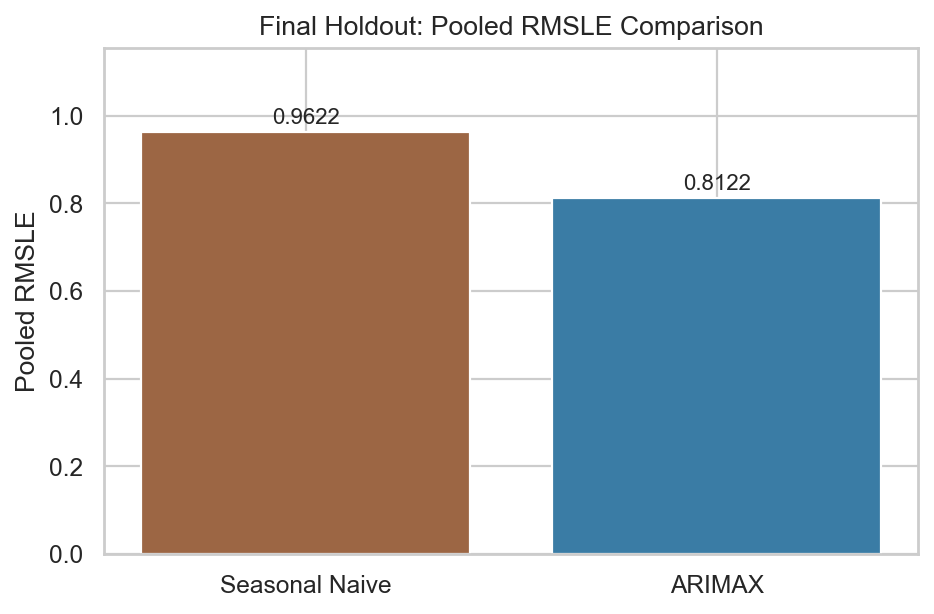
\includegraphics[width=0.78\textwidth]{figures/figure_rmsle_comparison.png}
  \caption{Final holdout pooled RMSLE comparison between Seasonal Naive and ARIMAX.}
\end{figure}

\begin{table}[H]
\centering
\caption{Main pooled forecast metrics on the final holdout}
\begin{tabular}{lccc}
\toprule
Model & RMSLE & RMSE$_{\log}$ & MAPE (\%) \\
\midrule
Seasonal Naive lag 7 & 0.9622 & 0.9622 & 131.82 \\
ARIMAX & 0.8122 & 0.8177 & 86.99 \\
\bottomrule
\end{tabular}
\end{table}

\subsection{Store-level consistency of the result}
The pooled result is reinforced by the store-level evidence. ARIMAX beats the baseline for 79.1\% of evaluated stores, which indicates that the improvement is not concentrated in a small number of restaurants. Instead, the gain appears across a clear majority of the store panel.

This point is important because the operational decision problem is inherently local. A restaurant manager cares less about whether a model improves an overall market average than about whether it improves forecasts for individual stores. A strong pooled result with a weak store-level win rate would therefore be less convincing. In contrast, the 79.1\% win rate suggests that the ARIMAX advantage is broadly distributed rather than narrowly driven.

Figure~2 provides a useful visual diagnostic of this pattern. The mass of the distribution lies to the right of zero, indicating that positive improvement is common across stores rather than being produced by a few extreme outliers. This does not imply universal dominance, but it does show that the pooled improvement and the store-level evidence point in the same direction.

\begin{figure}[H]
  \centering
  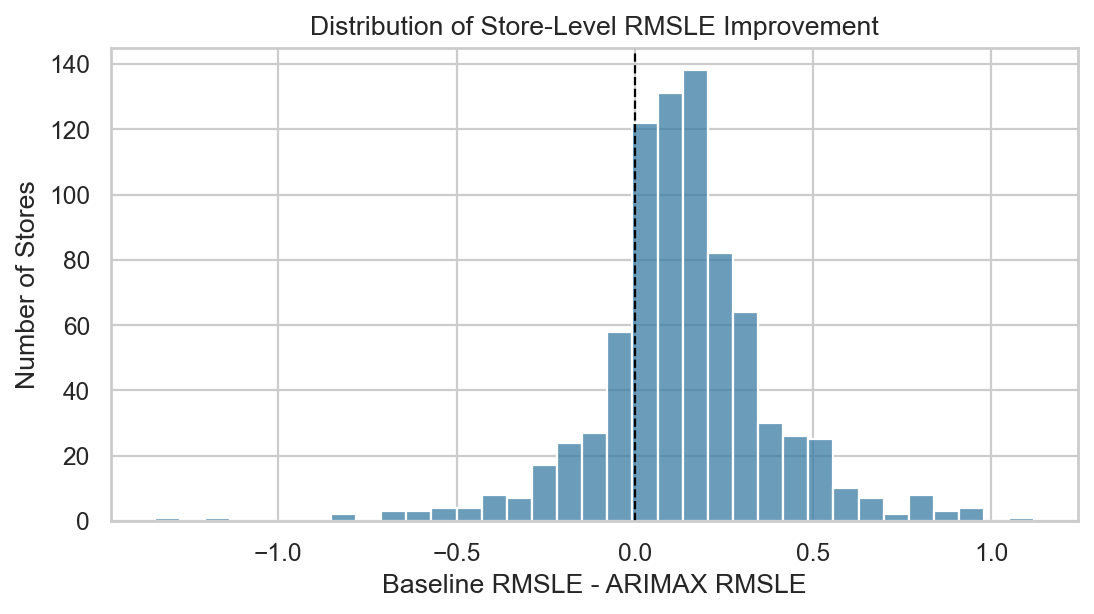
\includegraphics[width=0.85\textwidth]{figures/figure_store_improvement_distribution.png}
  \caption{Distribution of store-level RMSLE improvement, measured as baseline RMSLE minus ARIMAX RMSLE. Values above zero indicate that ARIMAX outperformed the benchmark.}
\end{figure}

\begin{table}[H]
\centering
\caption{Store-level summary of final holdout performance}
\begin{tabular}{lc}
\toprule
Statistic & Value \\
\midrule
Stores total & 814 \\
Stores evaluated & 812 \\
Stores skipped & 2 \\
Holdout observations & 31{,}476 \\
ARIMAX better than baseline & 79.1\% of evaluated stores \\
Improvement vs baseline & 15.6\% RMSLE reduction \\
ARIMAX fitting failures & 0 \\
\bottomrule
\end{tabular}
\end{table}

\subsection{Lightweight expanding-window validation result}
The project also includes one lightweight expanding-window validation fold before the final holdout. In that fold, training ends on 31 January 2017 and the test window covers 1 February to 7 February 2017. A total of 810 stores are evaluated, and the pooled validation set contains 5{,}670 store-date rows.

The validation result is directionally consistent with the final holdout. The Seasonal Naive baseline achieves RMSLE of 0.9327, while ARIMAX achieves RMSLE of 0.7317. This corresponds to a 21.6\% improvement, and ARIMAX beats the baseline for 69.4\% of evaluated stores in that fold.

This result should still be interpreted carefully. One lightweight expanding-window fold is not equivalent to a full multi-fold rolling-origin validation design, and it does not establish stability over all possible forecast origins. Its value is narrower: it shows that the ARIMAX advantage is not confined exclusively to one final March--April test window.

Methodologically, that matters because a single holdout can always raise the question of whether the result depends too heavily on the exact timing of the test period. The earlier fold does not eliminate that concern, but it reduces it. The report therefore uses the fold as supporting temporal evidence rather than as a substitute for broader validation.

\begin{table}[H]
\centering
\caption{Lightweight expanding-window validation fold}
\begin{tabular}{lc}
\toprule
Validation item & Value \\
\midrule
Train end & 2017-01-31 \\
Test window & 2017-02-01 to 2017-02-07 \\
Stores evaluated & 810 \\
Pooled rows & 5{,}670 \\
Seasonal Naive RMSLE & 0.9327 \\
ARIMAX RMSLE & 0.7317 \\
Improvement vs baseline & 21.6\% \\
ARIMAX better than baseline & 69.4\% of evaluated stores \\
\bottomrule
\end{tabular}
\end{table}

\subsection{Why ARIMAX improves over the baseline}
The improvement can be interpreted directly through the theoretical framework developed earlier. Seasonal Naive captures only one source of predictability: weekly repetition. It cannot respond to changing conditions such as public holidays, shifts in reservation demand, or store-specific dynamics that are not well represented by last week's same weekday alone.

ARIMAX improves because it combines three distinct forms of information. First, it uses autoregressive and moving-average terms to model store-specific persistence. Second, it includes explicit seasonal structure with a seven-day period. Third, it incorporates calendar and reservation variables that shift the forecast when known external conditions differ from those implied by weekly repetition alone. The result is a richer but still interpretable structure. Its gain does not come from opaque black-box flexibility; it comes from adding forecast-relevant information channels motivated by the economic logic of restaurant demand.

Figure~3 illustrates this idea at the store level. The purpose of the plot is not to prove that ARIMAX dominates on every date. Rather, it shows how the model can deviate from the weekly benchmark when actual demand departs from last week's pattern. That is precisely the setting in which the reservation and calendar channels should matter most.

\begin{figure}[H]
  \centering
  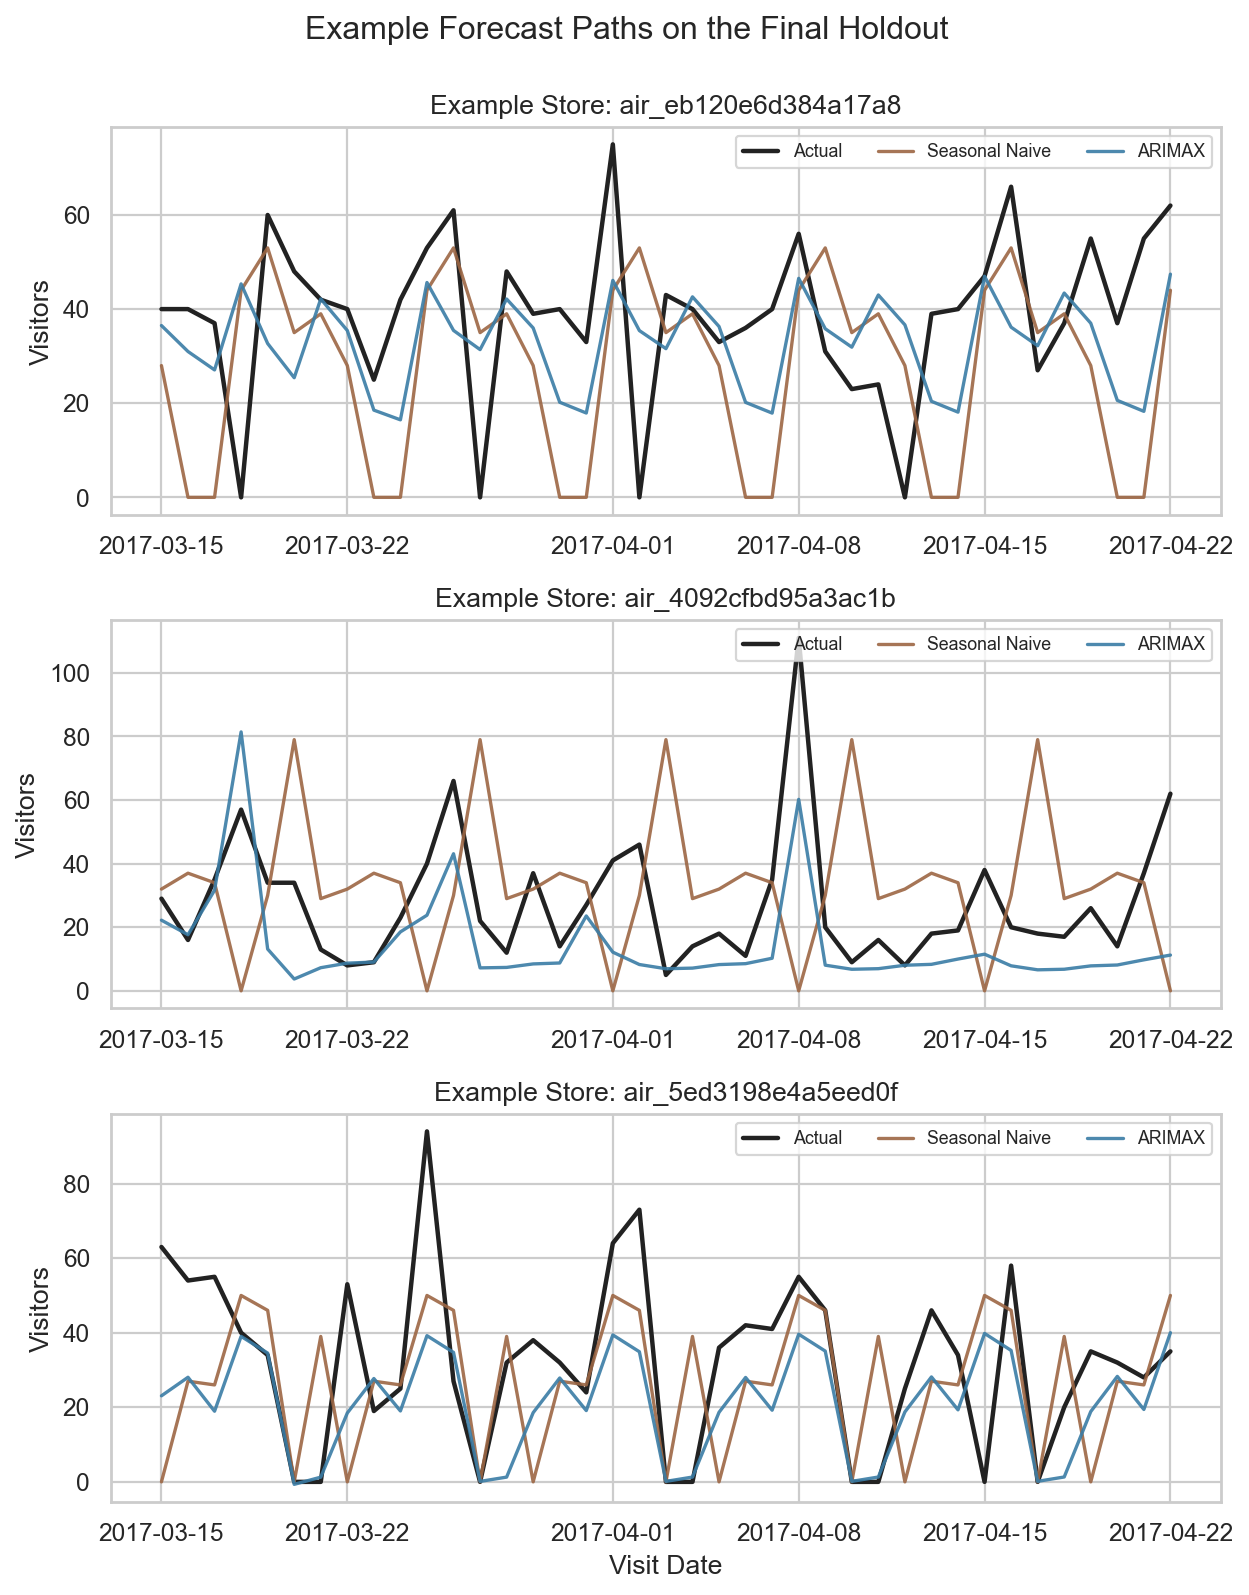
\includegraphics[width=0.88\textwidth]{figures/figure_example_forecasts.png}
  \caption{Example forecast paths for three stores on the final holdout window.}
\end{figure}

\subsection{What the results do not prove}
The results must be interpreted within the boundaries of the implemented design. They do not prove that ARIMAX is the best possible forecasting model across all alternatives, nor do they show that one final holdout plus one lightweight validation fold establishes universal stability across all forecast origins. They also do not directly validate Golden Week forecasting out of sample, because the final holdout does not cover the main Golden Week dates. These limitations do not invalidate the reported improvement, but they do define the proper scope of the claim.

\subsection{Interpreting the magnitude of the improvement}
The reduction in pooled RMSLE from 0.9622 to 0.8122 represents a meaningful gain because the comparator is already strong. Seasonal Naive is not a dummy baseline. It reflects a plausible weekly rule that many practical users could adopt without complex modelling, so beating it has substantive forecasting content.

The magnitude should nevertheless be interpreted comparatively rather than absolutely. A 15.6\% reduction in RMSLE does not imply that forecasts are close to perfect, and restaurant demand remains noisy because many relevant influences are not modelled explicitly. The defensible conclusion is narrower: across the evaluated store-date rows, ARIMAX makes smaller average log-scale errors than the weekly benchmark.

\subsection{Residual error interpretation and the role of MAPE}
MAPE remains high even after the ARIMAX improvement: 131.82\% for the baseline and 86.99\% for the final model. Those values can look discouraging at first glance, but they must be interpreted in the context of store-level restaurant data, where some stores and days have very low visitor counts. When actual demand is close to zero, even a small absolute error can translate mechanically into a very large percentage error. That feature is intrinsic to MAPE rather than unique to this project.

RMSLE is more appropriate here because it better reflects the scale heterogeneity of the forecasting problem. It reduces the influence of very large stores, accommodates zeros through the \texttt{log1p} transformation, and matches the idea that proportionate misprediction often matters more than raw absolute deviation in operational settings. A miss of eight visitors does not have the same economic meaning across all restaurants, and RMSLE handles that asymmetry better than a simple percentage measure.

For that reason, MAPE is retained mainly as a secondary descriptive diagnostic. Its directional movement is still informative: ARIMAX improves MAPE in the same direction as RMSLE, which is reassuring. But the substantive judgement of the paper rests on pooled RMSLE and store-level consistency, not on a metric known to become unstable in sparse count settings. This is a methodological choice grounded in the structure of the data rather than an ex post attempt to explain away an inconvenient result.

\section{Discussion}
\subsection{Operational implications}
The discussion begins from the practical reason the forecasting problem matters. Restaurant managers allocate labour, ingredients, and service capacity before realised demand is observed. In that environment, a forecast is valuable not because it eliminates uncertainty, but because it narrows the gap between expected and realised arrivals at the moment decisions must be made. The empirical results suggest that a model using store history, weekly seasonality, calendar variables, and reservations is more aligned with that planning problem than a benchmark that only repeats last week's pattern.

This practical interpretation is strongest at the store level. Underprediction can lead to understaffing, slower service, and stock-outs, while overprediction can lead to excess labour cost and food waste. Those consequences materialise locally rather than in the aggregate. A platform-level forecast may be useful for broad planning, but it cannot substitute for daily predictions at the individual restaurant level. In that sense, the store-level design is not simply a modelling choice; it is part of the report's practical interpretation of what forecast quality means.

Reservation information is especially important in this operational setting. Unlike many standard time-series regressors, reservations reflect commitments that exist before service begins. They therefore move the forecast closer to the real information set available to a manager at the planning stage. Calendar variables play a similar, though less direct, role. Weekends and holidays are known in advance and can shift expected customer behaviour even when recent weekly demand looks stable. The empirical value of ARIMAX is therefore consistent with a wider managerial intuition: forecasts improve when they incorporate information that decision-makers actually know before the day unfolds.

Golden Week should nevertheless be interpreted carefully. It is theoretically relevant because it is a major holiday period in Japan and can plausibly affect restaurant demand through travel, leisure, and family behaviour. Including \texttt{is\_golden\_week} is therefore reasonable as a calendar feature. However, the final holdout period ends on 22 April 2017, before the main Golden Week dates. In this report, Golden Week is best understood as a theoretically motivated calendar control rather than as a holiday effect that has been directly stress-tested out of sample.

\subsection{Limitations and future extensions}
The limitations of the study follow directly from its deliberately focused design. The first limitation is comparative scope. The project evaluates two implemented models: Seasonal Naive lag 7 and store-level ARIMAX. It does not run a broad model tournament involving Prophet, ETS, gradient boosting, random forests, LSTM, temporal fusion transformers, or hierarchical global models. That means the conclusion should remain proportional to the evidence: the report supports the claim that ARIMAX outperforms the implemented weekly benchmark, not the broader claim that it dominates the full forecasting model space.

The second limitation concerns temporal validation. The final chronological holdout and one lightweight expanding-window fold are appropriate for a forecasting design and avoid random-split leakage, but they do not establish performance across all possible forecast origins. Future work should apply additional rolling-origin or expanding-window splits to test whether the ARIMAX advantage remains stable under different seasonal regimes and different market conditions. This is the most direct path toward strengthening the temporal generality of the result.

The third limitation concerns panel construction. The notebook builds a complete daily frame within each store's observed span and fills missing internal dates as zero visitors in order to preserve the regular spacing required by the lag-7 benchmark and ARIMAX. This is a coherent operational rule, but it is still a modelling assumption rather than an economic observation. Future work could improve this part of the design by incorporating explicit store closure calendars, richer indicators of operating status, or alternative treatments of missing store-days.

The fourth limitation concerns model flexibility. The fixed ARIMAX order improves comparability, transparency, and reproducibility, but it may not be individually optimal for every store. Some restaurants may have dynamics that would be better captured by different orders or by models that borrow strength across similar stores. Future work could therefore compare the fixed-order design against automated per-store order selection, pooled panel models, hierarchical forecasting systems, or global models that explicitly learn across restaurants.

These limitations also point to a broader extension agenda. One direction is methodological: stronger rolling-origin validation, richer closure information, and alternative store-level or global forecasting architectures. Another direction is managerial: evaluating forecasting quality through explicit business costs such as labour shortages, excess staffing, waste, or service congestion rather than relying only on statistical error metrics. The latter extension would move the project from predictive accuracy toward decision analysis, which is the natural downstream application of the forecasting problem studied here.

Despite these limitations, the empirical design remains theoretically coherent. Demand is treated at the store level because the decision problem is store-specific. The benchmark uses lag 7 because weekly structure is central to restaurant demand. ARIMAX includes holiday, weekend, and Golden Week indicators because calendar conditions shift behaviour, and it includes \texttt{log1p\_reserve} because reservations reveal future demand in advance. The outcome is transformed with \texttt{log1p} and evaluated primarily with pooled RMSLE because the forecasting task involves non-negative, skewed, heterogeneous count data. Each major technical choice therefore follows from the economic and forecasting logic of the problem rather than being added ad hoc.

\section{Conclusion}
This report has presented a store-level forecasting study of daily restaurant visitors using the Recruit Restaurant Visitor Forecasting dataset. The implemented comparison is intentionally focused: a weekly Seasonal Naive lag-7 benchmark is evaluated against a store-level ARIMAX$(1,1,1)(1,1,1)[7]$ model with exogenous variables for holidays, weekends, Golden Week, and reservations. The forecasting unit is $\texttt{air\_store\_id} \times \texttt{visit\_date}$, and the central question is whether a dynamic regression design improves on a strong weekly benchmark when evaluation is conducted chronologically at the operational decision unit.

The evidence supports that narrower claim. On the final holdout, ARIMAX reduces pooled RMSLE from 0.9622 to 0.8122, corresponding to a 15.6\% improvement, and outperforms the benchmark for 79.1\% of evaluated stores. The lightweight expanding-window validation fold points in the same direction, with RMSLE improving from 0.9327 to 0.7317 and ARIMAX winning for 69.4\% of evaluated stores. These results are consistent with the theoretical argument of the report: restaurant demand is shaped not only by weekly repetition, but also by calendar structure and advance demand signals that are known before the visit date.

The conclusion remains deliberately disciplined. The project does not compare every possible forecasting model, does not directly validate Golden Week forecasting out of sample, and does not claim that one final holdout plus one lightweight validation fold establishes universal stability across all forecast origins. What it does show is more specific and therefore more credible: within the implemented store-level design, a fixed ARIMAX specification using calendar and reservation information adds forecasting value relative to a strong weekly Seasonal Naive benchmark.

That precision matters because empirical credibility depends on the match between evidence and claim. The report supports one coherent conclusion: when the forecasting problem is defined at the store-date level and the information set is restricted to what would have been known at the forecast origin, a dynamic regression model improves over a weekly seasonal benchmark. The argument does not need stronger language to be persuasive. Its strength comes from the consistency between the research question, the theoretical framework, the feature design, the evaluation strategy, and the reported results.

The broader implication is operational as well as statistical. Restaurant managers and platforms do not make decisions on aggregate market demand; they make decisions on individual stores and individual dates. A useful forecasting system should therefore respect the actual decision unit and exploit information that is available before service begins. Within the scope of this project, store-level ARIMAX provides a logical and empirically supported way to combine store history, weekly seasonality, calendar information, and reservation signals for that purpose.

\begin{thebibliography}{99}

\bibitem{boxjenkins1970}
Box, G. E. P., \& Jenkins, G. M. (1970).
\textit{Time Series Analysis: Forecasting and Control}.
San Francisco: Holden-Day.

\bibitem{boxtiao1975}
Box, G. E. P., \& Tiao, G. C. (1975).
Intervention analysis with applications to economic and environmental problems.
\textit{Journal of the American Statistical Association, 70}(349), 70--79.

\bibitem{hyndman2021}
Hyndman, R. J., \& Athanasopoulos, G. (2021).
\textit{Forecasting: Principles and Practice} (3rd ed.).
Melbourne: OTexts.

\bibitem{hyndmankoehler2006}
Hyndman, R. J., \& Koehler, A. B. (2006).
Another look at measures of forecast accuracy.
\textit{International Journal of Forecasting, 22}(4), 679--688.

\bibitem{makridakis2018}
Makridakis, S., Spiliotis, E., \& Assimakopoulos, V. (2018).
Statistical and machine learning forecasting methods: Concerns and ways forward.
\textit{PLOS ONE, 13}(3), e0194889.

\bibitem{tashman2000}
Tashman, L. J. (2000).
Out-of-sample tests of forecasting accuracy: An analysis and review.
\textit{International Journal of Forecasting, 16}(4), 437--450.

\bibitem{kaggle2017}
Kaggle. (2017).
\textit{Recruit Restaurant Visitor Forecasting}.
\url{https://www.kaggle.com/competitions/recruit-restaurant-visitor-forecasting}

\end{thebibliography}

\end{document}
